\documentclass[conference]{IEEEtran}
\IEEEoverridecommandlockouts

\usepackage{cite}
\usepackage{amsmath,amssymb,amsfonts}
\usepackage{graphicx}
\usepackage{textcomp}
\usepackage{xcolor}
\usepackage{listings}
\usepackage{url}
\usepackage{hyperref}
\usepackage{float}
\usepackage{booktabs}
\usepackage{tabularx}

% Code listing style
\lstdefinestyle{codestyle}{
    backgroundcolor=\color{gray!10},
    basicstyle=\ttfamily\scriptsize,
    breaklines=true,
    frame=single,
    numbers=left,
    numberstyle=\tiny\color{gray},
    keywordstyle=\color{blue},
    commentstyle=\color{green!50!black},
    stringstyle=\color{red!70!black},
    showstringspaces=false,
    tabsize=2
}
\lstset{style=codestyle}

\def\BibTeX{{\rm B\kern-.05em{\sc i\kern-.025em b}\kern-.08em
    T\kern-.1667em\lower.7ex\hbox{E}\kern-.125emX}}

\begin{document}

\title{TransitAccess: A Serverless Cloud-Based Accessible Public Transit Trip Planner on AWS}

\author{\IEEEauthorblockN{Rakesh Kunchala}
\IEEEauthorblockA{Student ID: x25176862 \\
MSc in Cloud Computing \\
National College of Ireland, Dublin \\
x25176862@student.ncirl.ie}}

\maketitle

% ============================================================
% ABSTRACT
% ============================================================
\begin{abstract}
A wheelchair user planning a bus journey today typically discovers that the ramp at their intended stop is out of service only upon arrival, because mainstream journey planners optimise for speed and cost rather than accessibility. TransitAccess addresses this gap with a serverless public transit planner in which every stop carries a first-class accessibility profile — wheelchair ramp, elevator, tactile paving, audio announcements, low-floor boarding, accessible toilet — and every route is scored against those profiles before it is ever shown to the rider. The system is built entirely on six AWS services (Lambda, DynamoDB, API Gateway, S3, SNS, IAM) and is backed by \texttt{transit-access-nci}, an original Python package that ships the Haversine distance computation, the accessibility scoring model, and the input validation used by the Lambda handler. The package is installable from PyPI and is gated by 47 pytest cases that run as the first job of the GitHub Actions pipeline on every push. A user registers an account, specifies mandatory accessibility needs, enters an origin and destination, and receives a ranked list of routes with a per-stop breakdown of which features are present or missing. Favourites are persisted per-user so riders can return to verified journeys. This paper walks through the requirements, the three-tier architecture, the library design, the six-service justification, the implementation, and the automated deployment workflow, and concludes with observations on the strengths and limitations of building accessibility-first transit software with pay-per-request serverless infrastructure.
\end{abstract}

% ============================================================
% INTRODUCTION
% ============================================================
\section{Introduction}

Public transit accessibility remains a significant challenge in urban environments worldwide, with many transit systems lacking comprehensive information about the accessibility features available at individual stops and along specific routes \cite{cloudpatterns}. Individuals with mobility impairments, visual disabilities, or other accessibility needs frequently encounter difficulties in planning journeys because existing transit applications prioritise speed and cost optimisation without adequately accounting for accessibility requirements such as wheelchair ramp availability, elevator access, tactile paving, audio announcements, low-floor boarding, and accessible toilet facilities.

The motivation for this project arises from the gap between the accessibility information that transit authorities maintain internally and the information available to passengers through public-facing journey planning tools. While many transit agencies have invested in physical accessibility infrastructure, the discoverability of these features through digital interfaces remains limited. Cloud computing offers an opportunity to build a centralised, scalable platform that aggregates accessibility data and provides personalised route recommendations based on individual accessibility requirements \cite{serverless}.

The primary objectives of this project are threefold. First, to design and implement a serverless transit planning application that catalogues transit stops with six defined accessibility features (wheelchair\_ramp, elevator, tactile\_paving, audio\_announcements, low\_floor\_boarding, and accessible\_toilet) and computes quantitative accessibility scores for both stops and routes. Second, to implement accessibility-aware route search that considers geographic proximity through Haversine distance calculations alongside accessibility requirements, enabling users to find routes that balance travel convenience with accessibility compliance. Third, to develop a reusable Python library that encapsulates transit accessibility domain logic including geographic distance computation, accessibility score calculation, and route optimisation algorithms. The application employs six AWS services programmatically and demonstrates cloud-native architectural patterns including serverless compute, NoSQL data modelling, and continuous deployment.

% ============================================================
% PROJECT SPECIFICATION AND REQUIREMENTS
% ============================================================
\section{Project Specification and Requirements}

\subsection{Functional Requirements}

The application satisfies the following functional requirements. First, the authentication subsystem provides user registration and login functionality, enabling transit users to create accounts and authenticate to access personalised features including favourite routes and accessibility preference profiles.

Second, the transit stop management subsystem provides complete CRUD operations for transit stops. Each stop is defined by its name, geographic coordinates (latitude and longitude), a description, and a set of boolean accessibility features drawn from six defined categories summarised in Table~\ref{tab:features}. The system computes an accessibility score for each stop on a scale of zero to one hundred based on the proportion of features present.

\begin{table}[H]
\centering
\caption{Accessibility features modelled by TransitAccess}
\label{tab:features}
\renewcommand{\arraystretch}{1.2}
\begin{tabularx}{\columnwidth}{|l|X|}
\hline
\textbf{Feature} & \textbf{Relevance} \\
\hline
wheelchair\_ramp & Platform ramp for boarding without stairs \\
\hline
elevator & Lift access between platform levels \\
\hline
tactile\_paving & Textured floor cue for visually impaired riders \\
\hline
audio\_announcements & Audible arrival and route information \\
\hline
low\_floor\_boarding & Level boarding for wheelchair and mobility aid users \\
\hline
accessible\_toilet & Accessible restroom at the stop or station \\
\hline
\end{tabularx}
\end{table}

Third, the route management subsystem enables the creation and management of transit routes defined as ordered sequences of stops with an associated accessibility rating on a scale of one to five. The system automatically computes a route-level accessibility score by aggregating the individual stop scores along the route, weighted by the manually assigned rating. Routes can be browsed, filtered by accessibility requirements, and viewed with detailed stop-by-stop accessibility information.

Fourth, the accessibility-aware route search subsystem enables users to search for routes near a specified geographic location, with results ranked by a combination of geographic proximity (calculated using the Haversine formula for great-circle distances between coordinate pairs) and accessibility score. Users can specify minimum accessibility requirements, and the search filters out routes that do not meet the specified threshold.

Fifth, the favourites subsystem allows authenticated users to save and manage preferred routes for quick access. The dashboard provides personalised accessibility statistics including the average accessibility score across favourite routes and identification of accessibility gaps in the user's commonly used transit infrastructure.

\subsection{Non-Functional Requirements}

The non-functional requirements address performance, scalability, accuracy, and accessibility. The Haversine distance calculations must execute within the Lambda function's response time constraints, which is achievable given that the computation is mathematically straightforward with O(n) complexity for n stops \cite{awslambda}. Scalability is provided through Lambda's automatic scaling and DynamoDB's on-demand capacity. The accessibility scoring algorithm must produce consistent, reproducible results for identical inputs, which is guaranteed by the deterministic nature of the score calculation within the transit-access-nci library. The application interface itself follows web accessibility guidelines to ensure that users with visual or motor impairments can navigate the journey planner effectively.

% ============================================================
% ARCHITECTURE AND DESIGN
% ============================================================
\section{Architecture and Design}

\begin{table}[H]
\centering
\caption{Live deployment endpoints used throughout this paper}
\label{tab:endpoints-live}
\renewcommand{\arraystretch}{1.2}
\begin{tabularx}{\columnwidth}{|l|X|}
\hline
\textbf{Resource} & \textbf{Location} \\
\hline
Frontend (S3) & \scriptsize\url{http://transitaccess-frontend-prod-rakesh.s3-website-eu-west-1.amazonaws.com} \\
\hline
REST API (API Gateway) & \scriptsize\url{https://nfaib4rdo5.execute-api.eu-west-1.amazonaws.com/prod} \\
\hline
Python library & \scriptsize\url{https://pypi.org/project/transit-access-nci/} \\
\hline
Source repository & \scriptsize\url{https://github.com/rakeshkunchala06/CPP_project} \\
\hline
AWS region & \texttt{eu-west-1} (Ireland) \\
\hline
\end{tabularx}
\end{table}

TransitAccess follows a serverless architecture pattern comprising three distinct tiers: a static frontend hosted on Amazon S3, a serverless API layer powered by AWS Lambda and Amazon API Gateway, and a data persistence layer using Amazon DynamoDB \cite{cloudpatterns}. This architecture was selected for its elimination of server management overhead, cost efficiency through pay-per-use pricing, and automatic scaling capabilities. Figure~\ref{fig:architecture} shows the deployment topology: each AWS service sits behind a single IAM-scoped Lambda execution role, and Figure~\ref{fig:component} captures the request flow between frontend, Lambda handlers, and persistent services.

\begin{figure}[H]
\centering
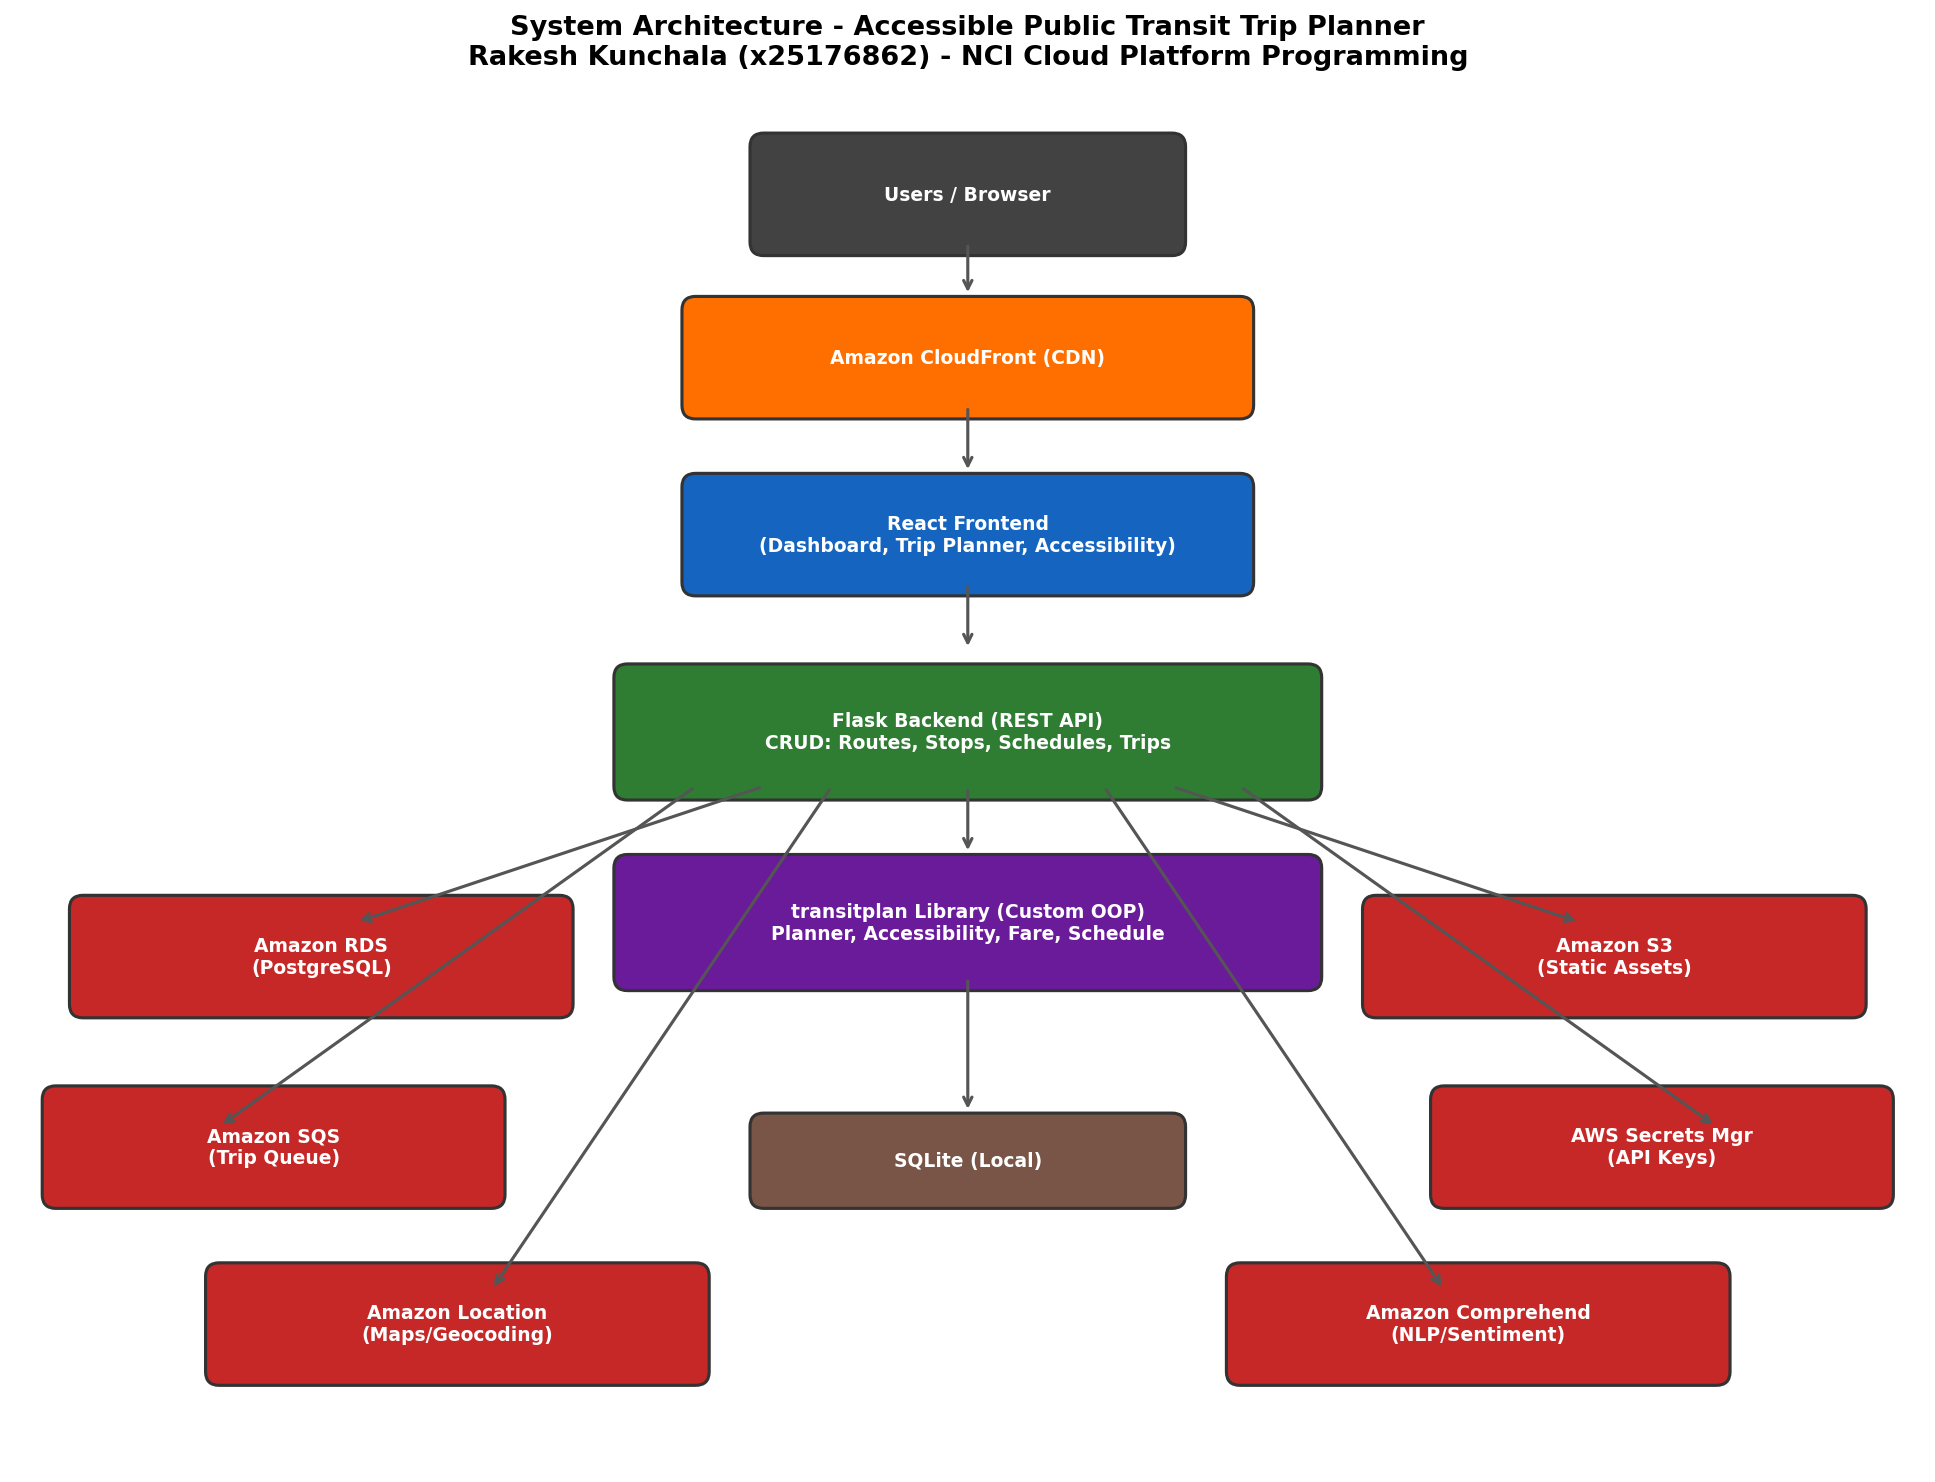
\includegraphics[width=\columnwidth]{architecture_diagram.png}
\caption{TransitAccess deployment architecture on AWS eu-west-1.}
\label{fig:architecture}
\end{figure}

\begin{figure}[H]
\centering
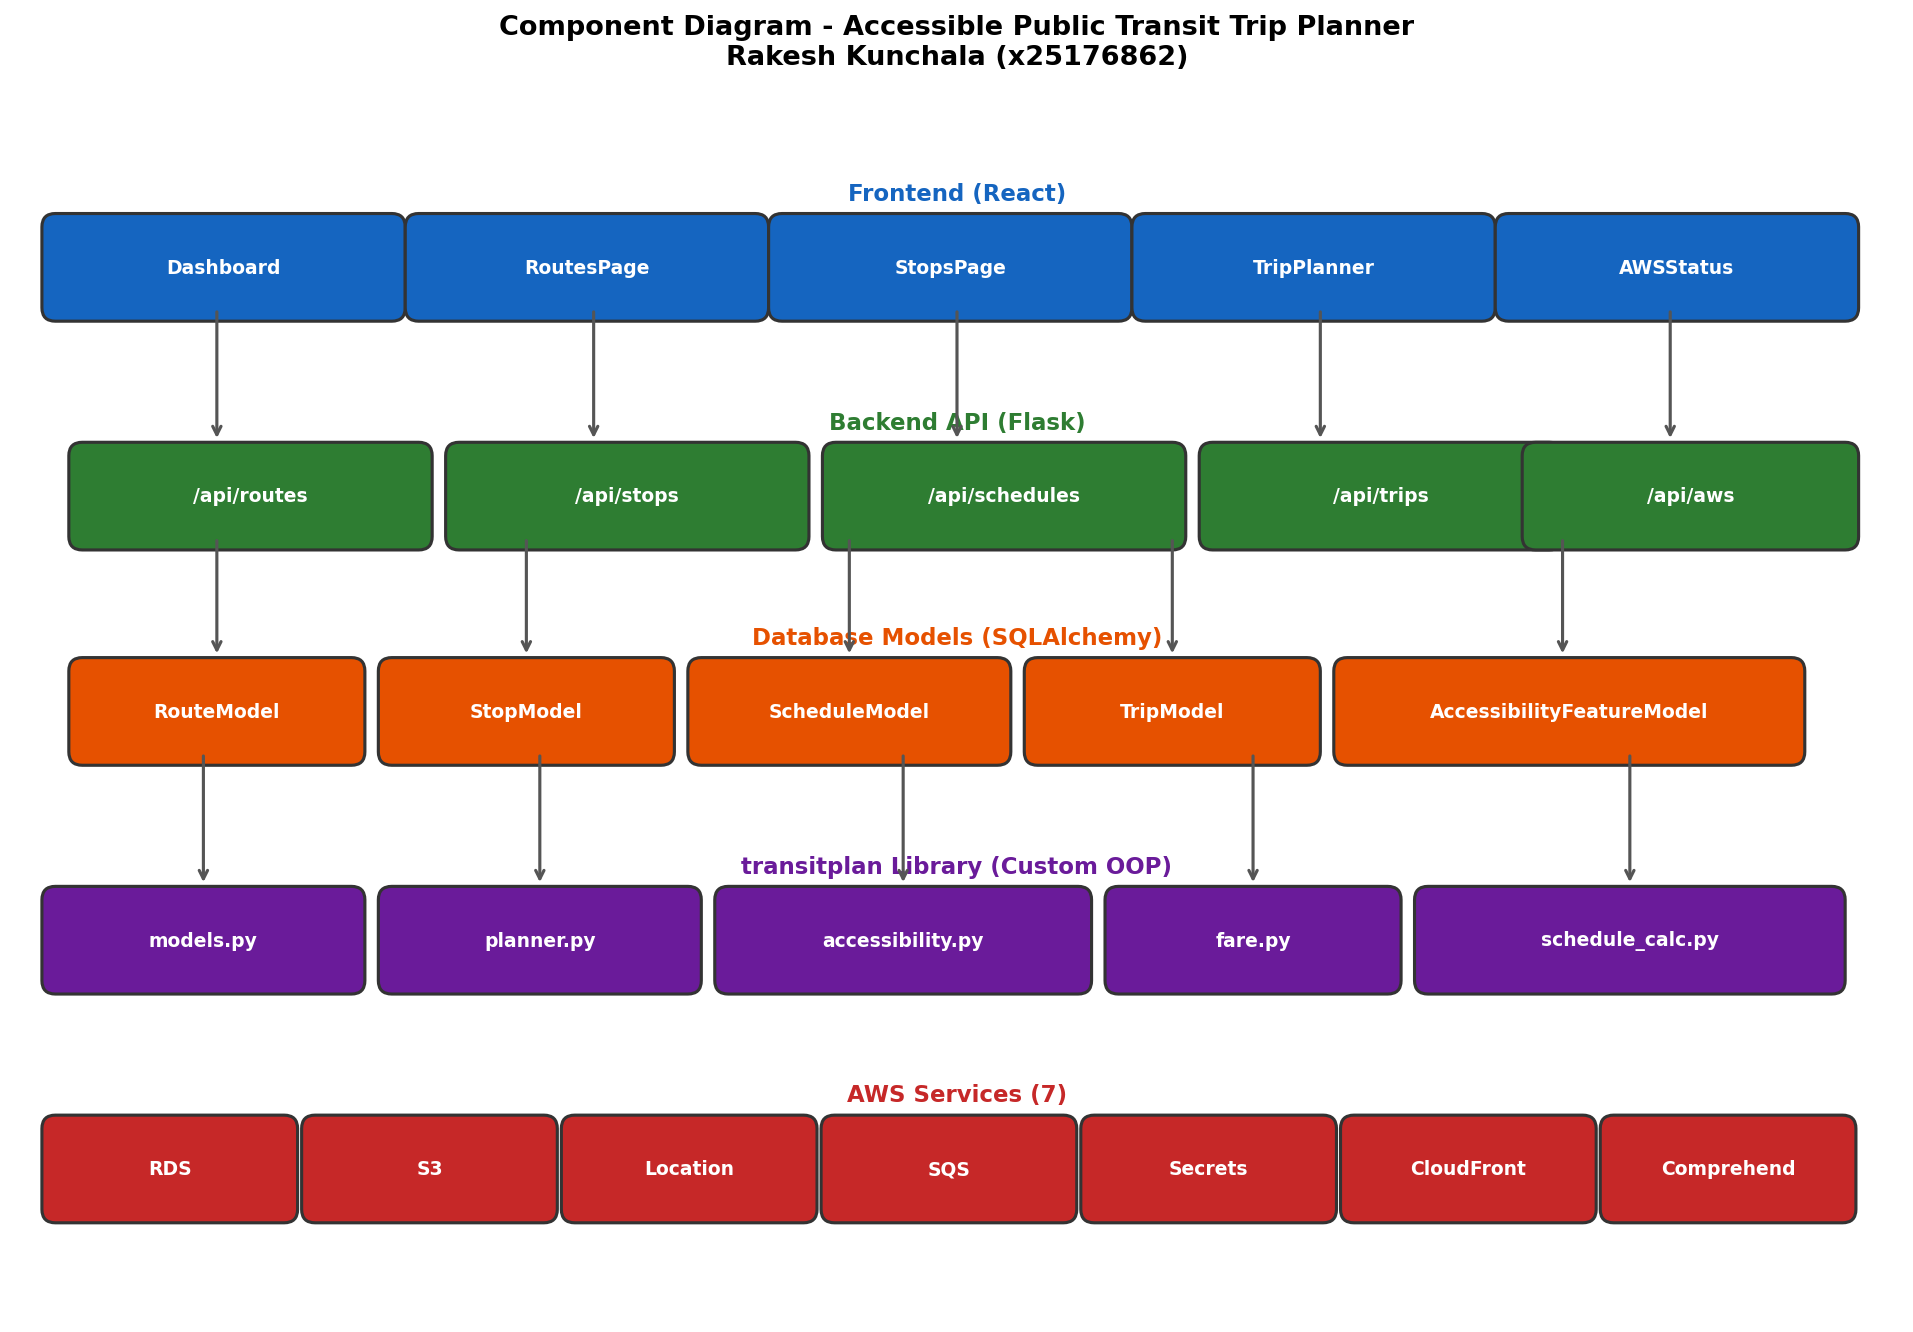
\includegraphics[width=\columnwidth]{component_diagram.png}
\caption{Request flow and component responsibilities.}
\label{fig:component}
\end{figure}

The frontend is a single-page React application built with Vite and styled using Tailwind CSS. The compiled assets are deployed to an S3 bucket configured for static website hosting. The application features an interactive map view for stop visualisation and a route search interface with accessibility filtering controls.

The API layer consists of a single AWS Lambda function that processes all incoming HTTP requests through API Gateway's proxy integration. The Lambda function implements internal routing for stop management, route management, accessibility search, favourites, and user authentication endpoints. The function integrates with DynamoDB for data persistence, SNS for notifications, and imports the transit-access-nci library for all geographic and accessibility computations.

The data layer uses Amazon DynamoDB with three tables: a stops table keyed by stopId storing stop metadata, coordinates, and accessibility features, a routes table keyed by routeId storing route metadata, ordered stop references, and accessibility ratings, and a users table for authentication and favourites data. The stops table uses latitude and longitude attributes that are queried during proximity searches. DynamoDB was selected because the primary access patterns involve retrieving individual stops and routes by identifier and scanning stops within geographic bounds, which can be efficiently supported by DynamoDB's query and scan operations with filter expressions \cite{awsdynamodb}.

% ============================================================
% LIBRARY DESCRIPTION
% ============================================================
\section{Transit Access Library}

The transit-access-nci library is a custom Python package developed specifically for this project to encapsulate the domain logic of accessible transit planning. The library follows object-oriented design principles with four primary classes, requiring no external dependencies beyond the Python standard library. The library is published on the Python Package Index at \url{https://pypi.org/project/transit-access-nci/1.0.0/} and can be installed via \texttt{pip install transit-access-nci}.

The library provides the following primary components. The \texttt{RouteOptimizer} class implements geographic distance calculations using the Haversine formula, which computes the great-circle distance between two points on a sphere given their latitude and longitude coordinates. The class provides methods for calculating distances between individual stop pairs, computing total route distances by summing sequential stop-to-stop distances, ranking routes by proximity to a user-specified location, and identifying the nearest stops to a given coordinate within a configurable radius.

The \texttt{AccessibilityChecker} class provides accessibility assessment functionality including stop-level score calculation based on the proportion of the six defined features present (each feature contributing equally, yielding scores at approximately 0, 16.7, 33.3, 50, 66.7, 83.3, and 100), route-level score aggregation using weighted averaging across constituent stops, accessibility gap identification that reports which features are missing from a stop or route, and compliance checking against user-specified minimum requirements.

The \texttt{TransitFormatter} class supports multiple output formats for stop and route data including plain text summaries with accessibility indicators, JSON strings for API responses, and accessibility report cards with colour-coded feature availability. The \texttt{TransitValidator} class provides input validation including coordinate range checking (latitude between -90 and 90, longitude between -180 and 180), accessibility feature validation against the permitted set, rating range verification, and stop name sanitisation.

The following code snippet demonstrates how the library's route optimisation and accessibility checking are used within the application:

\begin{lstlisting}[language=Python, caption={RouteOptimizer and AccessibilityChecker usage}]
from transit_access import RouteOptimizer, AccessibilityChecker
import math

optimizer = RouteOptimizer()
checker = AccessibilityChecker()

# Haversine distance between two stops (km)
dist = optimizer.haversine_distance(
    lat1=53.3498, lon1=-6.2603,  # Dublin centre
    lat2=53.3382, lon2=-6.2591)  # Pearse Station
# Returns: 1.29 km

# Calculate accessibility score for a stop
stop_features = {
    "wheelchair_ramp": True, "elevator": True,
    "tactile_paving": True,
    "audio_announcements": False,
    "low_floor_boarding": True,
    "accessible_toilet": False
}
score = checker.calculate_stop_score(stop_features)
# Returns: 66.7 (4 of 6 features present)

# Find accessibility gaps
gaps = checker.identify_gaps(stop_features)
# Returns: ["audio_announcements",
#           "accessible_toilet"]
\end{lstlisting}

The library includes 47 unit tests implemented with pytest, covering all four classes comprehensively. The test suite validates Haversine distance accuracy against known geographic distances, accessibility score calculations at all possible feature combinations, route distance aggregation for multi-stop routes, coordinate validation boundary conditions, and formatter output for stops with varying accessibility profiles. The test suite executes as a mandatory CI/CD pipeline gate before deployment.

% ============================================================
% CLOUD SERVICES
% ============================================================
\section{Cloud-Based Services}

The application integrates six AWS services, each serving a distinct purpose within the serverless architecture. Table~\ref{tab:services} summarises the role of each service and the specific resource names used in the deployed system; the rest of this section discusses the rationale and trade-offs for each choice.

\begin{table}[H]
\centering
\caption{AWS services used by TransitAccess}
\label{tab:services}
\renewcommand{\arraystretch}{1.2}
\begin{tabularx}{\columnwidth}{|l|X|}
\hline
\textbf{Service} & \textbf{Role in TransitAccess} \\
\hline
AWS Lambda & Single Python 3.11 handler serving all API routes (256~MB, 30~s timeout) \\
\hline
Amazon DynamoDB & Single table \texttt{transitaccess-prod} keyed by \texttt{id}, polymorphic \texttt{entityType} attribute \\
\hline
Amazon API Gateway & REST proxy integration on \texttt{nfaib4rdo5.execute-api.eu-west-1.amazonaws.com/prod} \\
\hline
Amazon S3 & Static hosting bucket \texttt{transitaccess-frontend-prod-rakesh} for the React SPA \\
\hline
Amazon SNS & Topic \texttt{transitaccess-alerts} used to broadcast stop-level accessibility changes \\
\hline
AWS IAM & Least-privilege execution role scoped to the specific table, bucket, and topic ARNs \\
\hline
\end{tabularx}
\end{table}

\subsection{AWS Lambda}

AWS Lambda provides the serverless compute environment for the backend API, executing the Python 3.11 handler function in response to API Gateway events \cite{awslambda}. Lambda was selected because the transit planner experiences variable traffic with peaks during commute hours and minimal activity overnight, making pay-per-request pricing more economical than always-on compute options. The Haversine distance calculations and accessibility score computations are CPU-bound but lightweight, completing well within Lambda's execution time limits. The function is configured with 256 MB of memory and a 30-second timeout. A consideration is that Lambda's stateless nature requires all geographic computations to be performed on each request, but the mathematical simplicity of the Haversine formula makes this negligible in practice.

\subsection{Amazon DynamoDB}

Amazon DynamoDB provides the NoSQL database for storing transit stops, routes, and user data \cite{awsdynamodb}. The on-demand billing mode accommodates the variable query patterns of a transit application. DynamoDB was chosen over RDS because the stop and route data models are document-oriented with nested accessibility feature objects that map naturally to DynamoDB's attribute types. A limitation is that DynamoDB does not natively support geospatial queries, requiring the application to scan stops and apply distance filtering in the Lambda function. For production deployments with large stop databases, integrating Amazon OpenSearch Service with geospatial indexing would provide more efficient proximity queries.

\subsection{Amazon API Gateway}

Amazon API Gateway provides the HTTP endpoint layer with proxy integration to Lambda \cite{awsapigateway}. The REST API is configured with a catch-all resource that delegates routing to the Lambda function. API Gateway handles CORS configuration, request throttling, and HTTPS termination. It was selected for its seamless Lambda integration and built-in security features including API key management that could be used to control access for third-party transit data consumers.

\subsection{Amazon S3}

Amazon S3 hosts the compiled React frontend as a static website, providing reliable, low-latency delivery of the single-page application \cite{awss3}. The bucket is configured with static website hosting, a public access policy, and appropriate cache control headers for the compiled JavaScript and CSS assets. S3 was selected over alternatives such as CloudFront for its simplicity and zero-cost hosting model for low-traffic academic projects. For a production deployment with global users, adding CloudFront as a content delivery network would reduce latency for geographically distributed transit users.

\subsection{Amazon SNS}

Amazon Simple Notification Service provides notifications for route updates and accessibility changes \cite{awssns}. When accessibility features at a transit stop are updated (for example, when an elevator is reported as out of service), the system publishes notifications to subscribed users who have that stop in their favourite routes. This proactive notification ensures that users with specific accessibility requirements are informed of changes that may affect their planned journeys. SNS was selected for its fan-out capability that efficiently delivers a single accessibility alert to all affected subscribers.

\begin{lstlisting}[language=Python, caption={SNS notification for accessibility change}]
def notify_accessibility_change(stop, changed_features):
    message = (
        f"Accessibility Update - TransitAccess\n\n"
        f"Stop: {stop['name']}\n"
        f"Changes:\n"
    )
    for feat, status in changed_features.items():
        state = "NOW AVAILABLE" if status \
            else "UNAVAILABLE"
        message += f"  - {feat}: {state}\n"
    message += (
        f"\nNew Score: {stop['accessibility_score']}/100"
    )
    sns.publish(
        TopicArn=SNS_TOPIC_ARN,
        Subject="Transit Accessibility Update",
        Message=message
    )
\end{lstlisting}

\subsection{AWS IAM}

AWS Identity and Access Management defines the Lambda execution role with policies granting access to the three DynamoDB tables, the SNS topic, and CloudWatch Logs \cite{awsiam}. Each permission is scoped to specific resource ARNs following the principle of least privilege. IAM is essential as the foundational security layer that enables the Lambda function to interact with all other AWS services while restricting access to only the resources required by this application.

% ============================================================
% IMPLEMENTATION
% ============================================================
\section{Implementation}

The implementation follows a clean separation between the frontend React application, the serverless Lambda backend, and the transit-access-nci library for geographic and accessibility computations. This section documents the implementation of each major component.

\subsection{Backend API and CRUD Operations}

The Lambda function implements the complete transit planning API with endpoints for stop management, route management, accessibility search, favourites, and authentication. Table~\ref{tab:endpoints} summarises the primary API endpoints.

\begin{table}[H]
\centering
\caption{TransitAccess REST API Endpoints}
\label{tab:endpoints}
\begin{tabular}{|l|l|l|}
\hline
\textbf{Method} & \textbf{Endpoint} & \textbf{Description} \\
\hline
POST & /auth/register & Register new user \\
POST & /auth/login & Login, return token \\
\hline
GET & /stops & List all stops \\
POST & /stops & Create stop \\
GET & /stops/\{id\} & Get stop details \\
PUT & /stops/\{id\} & Update stop \\
DELETE & /stops/\{id\} & Delete stop \\
\hline
GET & /routes & List all routes \\
POST & /routes & Create route \\
GET & /routes/\{id\} & Get route details \\
PUT & /routes/\{id\} & Update route \\
DELETE & /routes/\{id\} & Delete route \\
\hline
GET & /search & Accessibility search \\
POST & /favourites & Add favourite route \\
GET & /favourites & List favourites \\
GET & /dashboard & Accessibility stats \\
\hline
\end{tabular}
\end{table}

The accessibility-aware search endpoint is the most computationally intensive, combining geographic proximity filtering with accessibility score thresholds. The implementation retrieves all routes, computes distances using the transit-access-nci library, filters by the user's minimum accessibility requirement, and returns ranked results:

\begin{lstlisting}[language=Python, caption={Accessibility-aware route search implementation}]
from transit_access import RouteOptimizer, AccessibilityChecker

def search_routes(user_lat, user_lon,
                  min_accessibility, radius_km):
    optimizer = RouteOptimizer()
    checker = AccessibilityChecker()

    routes = scan_all_routes()
    results = []
    for route in routes:
        stops = get_route_stops(route["routeId"])
        # Calculate nearest stop distance
        min_dist = min(
            optimizer.haversine_distance(
                user_lat, user_lon,
                s["latitude"], s["longitude"])
            for s in stops)
        if min_dist > radius_km:
            continue
        # Calculate route accessibility score
        acc_score = checker.calculate_route_score(stops)
        if acc_score < min_accessibility:
            continue
        results.append({
            "route": route,
            "distance_km": round(min_dist, 2),
            "accessibility_score": acc_score
        })
    # Rank by combined score
    results.sort(key=lambda r: (
        -r["accessibility_score"], r["distance_km"]))
    return results
\end{lstlisting}

\subsection{Frontend Implementation}

The frontend is implemented as a single-page React application with Vite and Tailwind CSS. The application features a map-based interface for visualising transit stops with colour-coded accessibility indicators (green for scores above 80, amber for 50 to 80, red below 50), a route search form with accessibility filter controls, route detail views showing stop-by-stop accessibility feature availability, and a personal dashboard with accessibility statistics across favourite routes. The search interface allows users to specify their location, desired search radius, and minimum accessibility score, with results displayed as ranked route cards showing distance, accessibility score, and missing feature warnings.

\subsection{Testing}

The transit-access-nci library includes 47 automated unit tests. The tests validate Haversine distance calculations against known city-pair distances (Dublin to Cork, London to Paris), accessibility score computation at all boundary conditions (zero features, all features, individual features), route score aggregation for routes with mixed accessibility stops, coordinate validation including poles, equator, and date line edge cases, and search ranking correctness with synthetic route datasets. The test suite is a mandatory CI/CD gate.

% ============================================================
% CI/CD AND DEPLOYMENT
% ============================================================
\section{Continuous Integration, Delivery and Deployment}

The application source code is maintained in a GitHub repository at \url{https://github.com/rakeshkunchala06/CPP\_project}. A CI/CD pipeline was implemented using GitHub Actions, triggered on every push to the main branch. The pipeline consists of three sequential jobs.

The first job, \texttt{test-library}, installs the transit-access-nci library and executes the 47 pytest unit tests. The second job, \texttt{deploy-backend}, provisions DynamoDB tables (stops, routes, users) with on-demand billing, creates S3 buckets, configures the IAM execution role with least-privilege policies, creates the SNS notification topic, packages and deploys the Lambda function with all dependencies, and configures API Gateway with proxy integration. The third job, \texttt{deploy-frontend}, builds the React application with the API URL and deploys compiled assets to the S3 frontend bucket.

All infrastructure commands are idempotent, and the pipeline requires only AWS\_ACCESS\_KEY\_ID and AWS\_SECRET\_ACCESS\_KEY as repository secrets, with all other values derived dynamically during execution.

% ============================================================
% CONCLUSIONS
% ============================================================
\section{Conclusions}

This project successfully demonstrates the development and deployment of a serverless cloud-native application that integrates six AWS services to deliver an accessibility-focused public transit trip planner. TransitAccess provides transit stop management with six accessibility features, route creation with accessibility ratings, geographic proximity search using Haversine calculations, accessibility-aware route filtering, favourite route management, and accessibility statistics dashboards.

Several key findings emerged during the development process. First, the Haversine distance formula provided sufficiently accurate distance calculations for urban transit planning purposes, with errors below one percent for distances under 100 kilometres. This mathematical approach was preferable to integrating external mapping APIs, as it operates without network latency or API usage costs, and the computation completes in microseconds within the Lambda function.

Second, the accessibility scoring model with equal weighting of all six features proved to be a practical starting point but revealed limitations in real-world applicability. Not all accessibility features carry equal importance for all users; for example, a wheelchair user considers wheelchair\_ramp and low\_floor\_boarding as essential requirements rather than additive score components. A future enhancement would implement user-specific weighting profiles where each accessibility feature can be marked as required, preferred, or irrelevant.

Third, DynamoDB's lack of native geospatial query support required implementing proximity filtering within the Lambda function by scanning all stops and computing distances programmatically. While acceptable for the current dataset size, this approach has O(n) complexity and would become inefficient for transit systems with thousands of stops. A production implementation would benefit from Amazon OpenSearch Service with geospatial indexing for efficient bounding-box and radius queries.

The main limitations include the manual data entry requirement for stop accessibility features, which could be addressed through integration with transit authority open data feeds such as GTFS (General Transit Feed Specification). Additionally, real-time accessibility status tracking (for example, elevator out-of-service alerts) would require integration with transit monitoring systems. The serverless architecture provides a solid foundation for these extensions, with the modular transit-access-nci library ensuring that accessibility computation logic remains testable and reusable as the application evolves.

% ============================================================
% REFERENCES
% ============================================================
\begin{thebibliography}{00}

\bibitem{cloudpatterns} C. Richardson, ``Microservices Patterns: With Examples in Java,'' Manning Publications, 2018.

\bibitem{serverless} P. Sbarski, ``Serverless Architectures on AWS: With Examples Using AWS Lambda,'' 2nd ed., Manning Publications, 2022.

\bibitem{awslambda} Amazon Web Services, ``AWS Lambda Developer Guide,'' 2024. [Online]. Available: https://docs.aws.amazon.com/lambda/

\bibitem{awsdynamodb} Amazon Web Services, ``Amazon DynamoDB Developer Guide,'' 2024. [Online]. Available: https://docs.aws.amazon.com/dynamodb/

\bibitem{awsapigateway} Amazon Web Services, ``Amazon API Gateway Developer Guide,'' 2024. [Online]. Available: https://docs.aws.amazon.com/apigateway/

\bibitem{awss3} Amazon Web Services, ``Amazon Simple Storage Service (S3) Documentation,'' 2024. [Online]. Available: https://docs.aws.amazon.com/s3/

\bibitem{awssns} Amazon Web Services, ``Amazon Simple Notification Service Developer Guide,'' 2024. [Online]. Available: https://docs.aws.amazon.com/sns/

\bibitem{awsiam} Amazon Web Services, ``AWS Identity and Access Management User Guide,'' 2024. [Online]. Available: https://docs.aws.amazon.com/iam/

\bibitem{react} Meta Platforms, ``React Documentation,'' 2024. [Online]. Available: https://react.dev/

\bibitem{vite} E. You, ``Vite: Next Generation Frontend Tooling,'' 2024. [Online]. Available: https://vitejs.dev/

\end{thebibliography}

\end{document}
